\documentclass[a4paper, titlepage]{article}
\usepackage{graphicx}
\usepackage{biblatex}
\usepackage{parskip}

\usepackage{listings}
\usepackage{xcolor}
\lstset{
  basicstyle=\ttfamily,
  columns=fullflexible,
  breaklines=true,
  postbreak=\raisebox{0ex}[0ex][0ex]{\color{red}$\hookrightarrow$\space}
}
\graphicspath{ {./Images/} }
\addbibresource{biblography.bib}
\setcounter{tocdepth}{4}

\title{Parser Documentation}
\author{Adam, Brandon Cann, Xin Wang \thanks{document compiled by Xin Wang}}
\date \today
\date{ \today \\ v1.0}

\setlength{\parskip}{1em}

\begin{document}
    \maketitle
    
    \tableofcontents
    \pagebreak
 
    \section{Introduction}
    \indent
    According to the provided project briefing, a netlist describing the circuit will be provided in a file using a reduced SPICE format. It is required by the team to formulate an approach to read the file and store the information in a comprehensible data structure. 
    \par
    This document will research the format of the SPICE netlist and explore the different approaches in storing the information a certain way. This document is primarily used for planning the most effective way to approach the problem
    as well as allowing fellow teammates to engage productively on a equal knowledge footing. 
    \section{Input (.cir) file}
    Source file for any version of SPICE has the following format \cite{spice}.
    \begin{quotation}
        {\fontfamily{qcr}\selectfont
            TITLE \par
            ELEMENT \par
            .MODEL STATEMENTS \par
            ANALYSIS COMMANDS \par
            OUTPUT COMMANDS \par
            .END \par
        }
    \end{quotation}

    \textbf{Important points to note:}
    \begin{itemize}
        \item First line {\fontfamily{qcr}\selectfont TITLE } is used as a title on output files.
        \item File must end with command {\fontfamily{qcr}\selectfont .END} followed by a new line.
        \item Comment begins with '*' which covers entire line.
    \end{itemize}

    \section{Netlist Element Format}
    A circuit description is called a \textbf{netlist} which consists of statements defining a each circuit element.
    \par
    Connections are described by naming nodes [Actually stored as numbers].
    \par
    Format of an element description is:
        $$\tt{<D><description> <n1> <n2> [value] [parameters]}$$
        \begin{itemize}
            \item $\tt{<D>}:$ A character that is a unique identifier for each type of support circuit component
            \item $\tt{<description>}$ A string without space e.g. 5
            \item $\tt{[value]}$: The value a circuit component takes e.g. 500 ohms
        \end{itemize}
    \par
    We have to consider the situation where the input syntax is correct but the circuit represented is wrong.
    To overcome this, we need a function to check if the circuit described is realistic. 

    \subsection{Passive Elements in {\fontfamily{qcr}\selectfont 'letter'}}
    Passive elements are composed of the following:
    \begin{itemize}
        \item Resistors: {\fontfamily{qcr}\selectfont R} $$ \tt R<description> <n1> <n2> <value> $$
        \item Capacitor: {\fontfamily{qcr}\selectfont C} where we can specify the initial value of C for transient analysis.$$ \tt C<description> <n1> <n2> <value> [ic=<value>] $$
        \item Inductor: {\fontfamily{qcr}\selectfont L} where we can specify the initial value of L for transient analysis.$$ \tt L<description> <n1> <n2> <value> [il=<value>] $$
    \end{itemize}

    \subsection{Independent Sources}
    \begin{itemize}
        \item Voltage Sources 
        \begin{center}
            $\tt V<description> <n1> <n2><value>$
        \end{center}
        \item Current Sources
        \begin{center}
            $\tt I<description> <n1> <n2><value>$
        \end{center}
    \end{itemize}

    \par
    The character after the letter must be a unique instance name and followed by the nodes associated with + and - respectively.
    \par
    \textbf {When users are entering component values, it is important that the software recognises common abbreviations for units.}

    \subsection{Support for powers of ten}
    In order to support {\fontfamily{qcr}\selectfont spice} format, the following abbreviations for powers of ten must be recognised:
    \begin{itemize}
        \item f [femto]: $ 10^{-15} $
        \item p [pico]: $ 10^{-12} $
        \item n [nano]: $ 10^{-9} $
        \item u [micro]: $ 10^{-6} $
        \item m [milli]: $ 10^{-3} $
        \item k [kilo]: $ 10^{+3} $
        \item M [mega]: $ 10^{+6} $
        \item G [giga]: $ 10^{+9} $
        \item T [tera]: $ 10^{+12} $
    \end{itemize}
    Any unrecognised characters are ignored.

    \section{Network Diagram/Graphs}
    Network Graphs show the relationships between a set of entries. Each entry is represented by a \textit{Node} and the connections between nodes are represented through \textit{Edges}.
    \par
    There are four main types of network graphs:
    \begin{itemize}
        \item Undirected and Unweighted
        \item Directed and Unweighted
        \item Undirected and Weighted
        \item Directed and Weighted
    \end{itemize}
    \par
    A graph $G=(V, E)$ consists of: \cite{parse}  % changed X to V for vertices and from U to E for edges
    \begin{itemize}
        \item a finite set $V = \left\{ x_1, x_2, \dots, x_n \right \}$ whose elements are called nodes or vertices % added underscore for index and changed { } to \{ \} for proper notation of sets
        \item a subset $E$ of the Cartesian product $V \times V$, the elements of which are called arcs. % changed x to \times
    \end{itemize}
    The network graph defined will consists of two vector structures:
    \begin{itemize}
        \item Vector of nodes in the circuit
        \item Vector of branches in the circuit
    \end{itemize}
    The theoretical output is an ordered vector of branches and an ordered vector of nodes. 
    \textbf{Position starts from 1 as node 0 indicates GND.}
    \par
    This area will be explored more in-depth in the analysis module.
    \pagebreak

    \section{Implementation}
    Block diagram depicting the breakdown of Parse Netlist module:
    \begin{figure}[h]
    \centering
    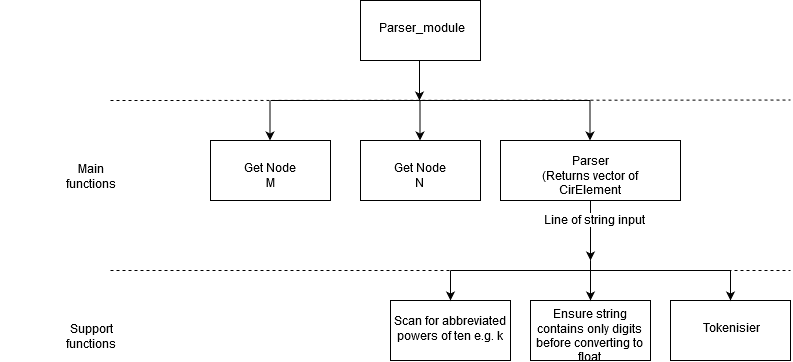
\includegraphics[width=145mm,scale=1]{Netlist breakdown}
    \caption{Netlist module breakdown}
    \label{fig:Netlist breakdown}
    \end{figure}
    \subsection{CirElement struct}
    \begin{lstlisting}[language=C++]
        CirElement 
        {
            variables:
    
                letter: component name
                name: name of node
                node1: node this node is connected to 
                node2: node this node is connected to
                value: float
                initial_val: float
        }
    \end{lstlisting}
    \subsection{Parser}
    \begin{lstlisting}[language=C++]
        parser(cin)
            {
                Tokenise
                Put in values into respective variables
                Detect values, pass into custom_pow
                Detect if initial_val is entered:
                    Pass into variable otherwise default 0
                Push CirElement into vector
            }
    \end{lstlisting}
    \subsubsection{custom pow}

    \begin{lstlisting}[language=C++]
        custom_pow(string: input)
            {
                Check if there are keywords e.g. k, m, M, G
    
                If not present, two scenario:
                    Unknown letter present: extract digits 
                    Convert to float
                    Empty string (End of recursion): return 0
    
                If present:
                    Find position where keyword appears
                    Take string before keyword and convert
                    Multiply/divide the digit by keyword
                    Recursion to cover case: 5M7k
            }
    \end{lstlisting}

    \subsubsection{tokeniser}
    \begin{lstlisting}[language=C++]
        tokeniser(string: input)
            {
                Call regex to tokenise the string 
                Push each token into a vector 
                Return vector
            }
    \end{lstlisting}

    \subsubsection{isdigit}
    \begin{lstlisting}[language=C++]
        isdigit(string: input)
            {
                Iterate over string
                Take each character and into 'isdigit' test
                Return boolean
            }
    \end{lstlisting}
    \subsection{Node N}
    \begin{lstlisting}[language=C++]
        getnodeN(vector<CirElement>: input)
        {
            Declare counter: M
            Find vector size: S
            Scan entire vector
            {
                Find times 'V' or 'I' occur
            }
            'N' is S - M
            Return N
        }
    \end{lstlisting}
    \subsection{Node M}
    \begin{lstlisting}[language=C++]
        getnodeN(vector<CirElement>: input)
        {
            Declare counter: M
            Scan entire vector
            {
                Find times 'V' or 'I' occur
            }
            Return M
        }
    \end{lstlisting}

    \pagebreak
    \section{Miscellaneous}
    There are more components to consider such as:
    \begin{itemize}
        \item Voltage controlled dependent sources
        \item Current controlled dependent sources
        \item Diodes
        \item BJT
        \item MOSFET
        \item Python implementation
        \item Efficient way to use recursion and not efficient to use matrix but more accurate.
    \end{itemize}


    \pagebreak
    \printbibliography[title={References}]

\end{document}